\section{Softwareudvikling AKA Greger er dum}
\subsection{Projektstyring}
Under de første møder til projektet, blev det aftalt at projektet skulle planlægges ved hjælp af sprints fra Scrum og at der skulle holdes jævnlige Scrum møder.
\newline
Der blev i starten af projektet derfor lavet en product backlog, hvori der blev angivet over hvor lang tid, hver eneste funktionalitet ville tage at implementere. Denne product backlog kan ses i BILLAG.
\newline
Sprintene skulle defineres ud fra, hvad der vil skabe mest værdi for projektet. Denne planlægning var tiltænkt at man kunne tilpasse projektarbejdet i forhold til undervisningen bedre. Derudover skulle sprints også laves på baggrund, for først at løse kravene og derefter visse udvalgte sekundære funktionaliteter.
\newline
Efter en sprint var defineret, ville der blive oprettet en Sprint backlog, som skulle dokumentere hvor meget arbejde der blev lagt i en problemstilling, og hvor meget workload der var tilbage. Sprint backloggen skulle derfor opdateres løbende under den pågældende sprint Sprint backlog'en fra uge 47-49 kan ses i figur \ref{fig:4749}:
\begin{figure}[ht]
	\centering
	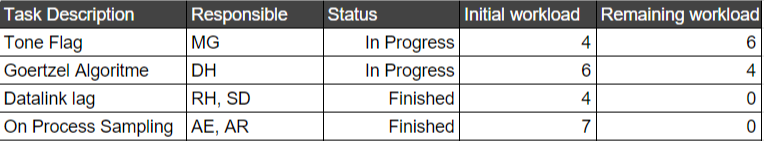
\includegraphics[width=15cm,height=25cm,keepaspectratio]{pictures/SprintBack47_49.png}
	\caption{Uge 47-49 sprint backlog}
	\label{fig:4749}
\end{figure}
\hfill \break

Yderlige eksempler på Sprint backlogs kan findes i BILAG.
\newline
Til Scrum møderne blev der udspecificeret en klar plan for, hvordan møderne skulle foregå, og hvilke elementer der skulle gennemgåes under møderne. I denne plan blev der også skrevet et kort teori afsnit, omkring hvordan man skal forholde sig til både Scrum møder og backlogs. Dette blev gjort med den hensigt, at hvert medlem ville være i stand til, at sikre at et Scrum møde blev udført korrekt og at backlogs blev opdateret.
\newline
Denne plan kan ses i BILLAG.

\subsection{Software Requirements Specification (SRS)}

\subsubsection{Idéudvikling}
Der blev i starten af projektet idéudviklet på den applikation der skulle laves. Der var flere idéer, hvorefter én blev valgt. Imellem disse idéer var en matematik applikation hvor en klient kunne sende et spørgsmål til en server og få et svar tilbage. Idéen var inspireret af Wolfram Alpha. Derudover var der også en idé, som til sidst blev valgt, som gik ud på at lave en chat applikation. Chat applikationen var inspireret af Skype, som fungerer på klient til klient plan. Der blev dog lagt op til at man kunne undersøge at lave en klient-server-klient hvis tiden var til det.
\hfill \break
Efter at have specificeret hvilken applikation der overordnet skulle laves, blev der lavet en brainstorm for krav til funktionaliteterne på applikationen, som kan ses på figur. 
\begin{figure}[ht]
	\centering
	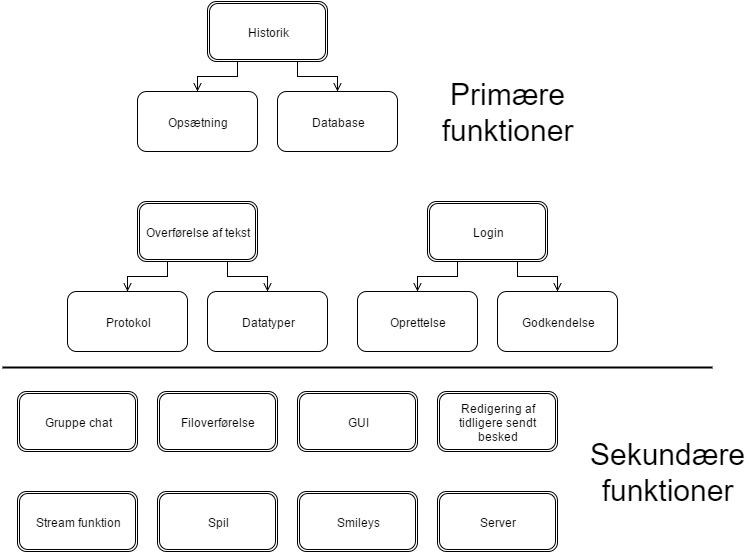
\includegraphics[width=15cm,height=25cm,keepaspectratio]{pictures/Ideudvikling.png}
	\caption{Brainstorm}
	\label{fig:brain}
\end{figure}
\newline
Som der ses på figur \ref{fig:brain} er funktionaliten delt op i to kategorier, primære- og sekundære funktioner. Hvor primære funktioner repræsenterer de funktionaliteter der minimum skal være i applikationen. De sekundære funktioner repræsenterer udvidelser som kan skabe værdi for brugeren.

\subsubsection{Kravspecifikation}
Udover at applikationen har nogle funktionaliteter, skal applikationen også have nogle krav. Disse krav er med til at opbygge applikationen og hjælper med at lede projektet mod en række problemstillinger der skal løses.
\newline
Kravene er som følger:
\begin{itemize}
	\item Sende beskeder mellem 2 applikationer
	
	\item Brugergrænseflade
	
	\item Pålidelig dataoverførsel
	
	\item Fejl testning af beskeder
	
	\item Se tidligere sendte og modtagede beskeder
	
	\item Login
\end{itemize}